\chapter{Das Lösungskonzept}
\label{cha:Lösungskonzept}
In diesem Kapitel wird der Lösungsansatz und die Spezifikation des Vorlagenmanagements erörtert. Bei der Spezifikation handelt es sich um Schnittstellen und abstrakte Klassen, die die Struktur des Vorlagenmanagements definieren. Diese Schnittstellen und abstrakten erlauben es Implementierungen für verschiedene \emph{Template-Engines} wie z.B
\begin{itemize}
	\item \emph{Freemakrer},
	\item \emph{Velocity} oder
	\item \emph{Thymeleaf}
\end{itemize}
zur Verfügung zu stellen, wobei die abstrakten Klassen die gemeinsam nutzbare Logik implementieren, die über die verschiedenen \emph{Template-Engines} verwendet werden kann.
\newline
\newline
Mit der Möglichkeit die verschiedensten \emph{Template-Engines} verwenden zu können, wird erreicht dass das Vorlagenmanagement sehr flexibel ist. Bei dem Wechsel zu einer anderen \emph{Template-Engine} müssen nur die \emph{Expressions} einer Vorlagen in die \emph{Template-Engine} spezifischen \emph{Expressions} umgewandelt werden. 

\section{Die Spezifikation der Vorlagen-\emph{API}}
Dieses Kapitel behandelt die erstellten Spezifikationen des Vorlagenmanagements. Auf Basis dieser Spezifikationen wird das Vorlagenmanagement und die Integrationen in die verschiedenen Umgebungen realisiert. Die erstellte Spezifikationen sind frei von Abhängigkeiten auf konkrete Implementierungen jeglicher Art. Sie haben nur Abhängigkeiten auf andere Spezifikationen wie die \emph{JEE-7} Spezifikation.
\begin{figure}[h]
\centering
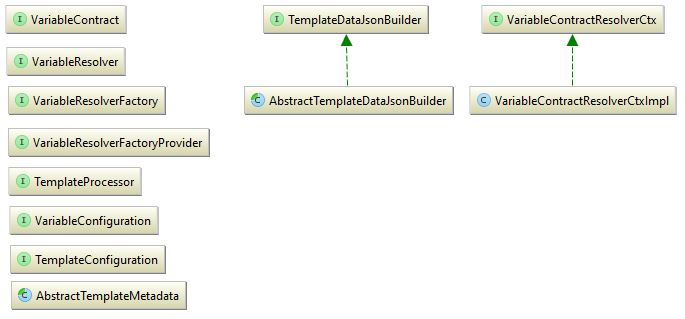
\includegraphics[scale=0.73]{20160710_template-logic-api.jpg} %{CS0031}
\caption{Klassenhierarchie der Vorlagen-\emph{API}}
\label{fig:template-logic-api-hierarchy}
\end{figure}
\ \newpage

\subsection{Die Schnittstellen und abstrakten Klassen}
Dieser Abschnitt behandelt die implementierten Schnittstellen und abstrakten Klassen des Vorlagenmanagements. Die abstrakten Klassen beinhalten die gemeinsam nutzbare Funktionalitäten, welche von alle konkreten Implementierungen des Vorlagenmanagements genutzt werden kann. Diese Spezifikationen spezifizieren folgende Aspekte des Vorlagenmanagements wie
\begin{enumerate}
	\item das Variablenmanagement innerhalb des Vorlagenmanagement,
	\item die Behandlung von Variablen in einer Vorlage 
	\item die Abbildung der Metadaten einer Voralge und 
	\item das Erstellen des \emph{JSON}-Objekts, welches die Daten für die Vorlage beinhaltet.
\end{enumerate}

\subsubsection{Die Schnittstelle \emph{VariableContract}}
\label{sec:variableContract}
Die Schnittstelle \emph{VariableContract} spezifiziert eine Variable, die in einer Vorlage verwendet werden kann. Objekte dieser Schnittstelle werden einmalig registriert und können in allen Vorlagen verwendet werden. Eine Variable ist einem Modul zugeordnet, in dem die Variable bezüglich ihres Namen eindeutig sein muss. Das Modul wird über einen \emph{String} definiert. Die Mehrsprachigkeit eines Variablenkontrakt wird über Enumerationen realisiert, wobei ein jeder Variablenkontrakt jeweils einen Schlüssel für den \emph{Label} und die Beschreibung bereit stellt. 
\newline
\newline
Da es sich bei einer Variablenkontrakt um statische Daten handelt, also die Variablen sind schon zur Kompilierungszeit bekannt sind, ist angedacht, dass die Variablen mit dem \emph{Java}-Typ \emph{enum} definiert werden, wobei in einer Klasse von Typ \emph{enum} mehrere Variablen definiert auf einmal werden können. Diese definierten Variablen innerhalb dieser Klasse sollten demselben Modul zugeordnet sein. Die Variablen, die mit einer \emph{enum} definiert wurden, werden innerhalb des Vorlagenmanagements trotzdem als einzelne Objekte der Schnittstelle \emph{VariableContract} betrachtet. Die Tatsache dass die Variablen mit einer \emph{enum} abgebildet wurden, ist für das Vorlagenmanagement nur beim Registrieren der variablen von belang und nicht bei deren weiterer Verwendung.
\newpage

\begin{program}[h]
\caption{VariableContract.java}
\label{prog:variableContract}
\begin{JavaCode}
public interface VariableContract extends Serializable {

    String getName();

    String getModule();

    Enum<?> getInfoKey();

    Enum<?> getLabelKey();

    default String getId() {      
		return getModule() + "." + getName();
    }

    default String toInfoString() {
        final String ls = System.lineSeparator();
        final StringBuilder sb = new StringBuilder();
        sb.append("contract  : ").append(this.getClass().getName())
          .append(ls)
          .append("id        : ").append(getId())
          .append(ls)
          .append("name      : ").append(getName())
          .append(ls)
          .append("label-key : ").append((getLabelKey() != null) 
                                          ? getLabelKey().name() 
                                          : "not available")
          .append(ls)
          .append("info-key  : ").append((getInfoKey() != null) 
                                          ? getInfoKey().name() 
                                          : "not available")
          .append(ls)
          .toString();
    }
}
\end{JavaCode}
\end{program}
\ \newline
Ein Variablenkontrakt ist über seine Id eindeutig referenzierbar, wobei sich die Id aus dem Modulnamen und den Variablennamen zusammensetzt (Bsp. module.core.VARIBALE).
Dieses Verhalten soll immer gleich sein, deswegen wurde die Methode \emph{String getId();} als \emph{default Methode} implementiert, was seit \emph{Java8} möglich ist. Ein EntwicklerIn muss diese Methode nicht mehr implementieren, obwohl es immer noch möglich ist diese Methode zu überschreiben. Auch die Methode \emph{String toInfoString()} wurde als \emph{default Methode} implementiert, da auch diese Methode nicht von den EntwicklerInnen implementiert werden sollte, da ihre Funktionalität nicht ändern sollte. 

\subsubsection{Die Schnittstelle \emph{VariableResolver}}
\label{sec:variableResolver}
Die Schnittstelle \emph{VariableResolver} spezifiziert wie Variablen aufgelöst werden. Eine Variable wird in einer Vorlage verwendet und beim Parsen dieser Vorlage muss der aktuelle Wert der Variable aufgelöst werden. Da dieser Variablenwert abhängig ist vom Kontext der Vorlage wird beim Auflösen der Variable ein Kontext bereitgestellt, über den kontextabhängige Daten vom EntwicklerIn bereitgestellt werden können, die in einer Implementierung der Schnittstelle \emph{VariableResolver} angewendet werden können. Dadurch könnte die Variable in mehreren Kontexten verwendet werden und auch unterschiedlich aufgelöst werden abhängig vom aktuell gesetzten Kontext.
\begin{program}[h]
\caption{VariableResolver.java}
\label{prog:variableResolver}
\begin{JavaCode}
@FunctionalInterface
public interface VariableResolver {

    String resolve(VariableContract variable,
                   VariableContractResolverContext ctx);
}
\end{JavaCode}
\end{program}
\ \newline
Die Schnittstelle wurde als \emph{FunctionalInterface} implementiert. Ein \emph{FunctionalInterface} ist eine Schnittstelle, die nur eine abstrakte Methode definiert, die implementiert werden muss. Eine Implementierung eines \emph{FunctionalInterface} kann über eine \emph{Lambda}-Funktion oder Methodenreferenzen bereitgestellt werden, wodurch die Notwendigkeit einer anonymen Implementierung oder der Implementierung einer Klasse wegfällt. Dieser Ansatz macht den Quelltext lesbarer, obwohl angemerkt sei, dass dieser Ansatz sich negativ auf das Laufzeitverhalten auswirkt, was in der Art und Weise der Ausführung einer \emph{Lambda}-Funktion begründet ist. Die negativen Auswirkungen auf das Laufzeitverhalten können im Bezug auf das Vorlagenmanagement vernachlässigt werden.

\subsubsection{Die Schnittstelle \emph{VariableResolverFactory}}
\label{sec:variableResolverFactory}
Die Schnittstelle \emph{VariableResolverFactory} spezifiziert wie Objekte der Schnittstelle \emph{VariableResolver} produziert werden. Objekte dieser Schnittstelle können Implementierungen der Schnittstelle \emph{variableResolver} für jede Art von Variablen produzieren, obwohl es zu empfohlen ist, dass es eine Implementierung der Schnittstelle \emph{VariableResolverFactory} je Variablenmodul gibt.
\newpage

\begin{program}[h]
\caption{VariableResolverFactory.java}
\label{prog:variableResolverFactory}
\begin{JavaCode}
@FunctionalInterface
public interface VariableResolverFactory extends Serializable {

  VariableResolver getVariableResolver(VariableContract contract,
                                       VariableContractResolverCtx ctx);
}
\end{JavaCode}
\end{program}
\ \newline
Auch diese Schnittstelle wurde als \emph{FunctionalInterface} implementiert, damit Implementierungen über \emph{Lambda}-Funktionen oder Methodenreferenzen bereitgestellt werden können.

\subsubsection{Die Schnittstelle \emph{VariableResolverFactoryProvider}}
\label{sec:VariableResolverFactoryProvider}
Die Schnittstelle \emph{VariableContractFactoryProvider} spezifiziert wie Objekte der Schnittstelle \emph{VariableResolverFacotry} produziert werden. Ein Objekt der Schnittstelle \emph{VariableResolverFactoryProvider} kann Objekte der Schnittstelle \emph{VariableResolverFactory} für eine konkrete Implementierung der Schnittstelle \emph{VariableContract} zur Verfügung stellen. Es ist angedacht, dass die Variablen mit dem \emph{Java}-Typ \emph{enum} definiert werden, wobei die Implementierung eines \emph{Enum}-Typs die Schnittstelle \emph{VariableContract} implementiert. Dadurch definiert jede einzelne Enumeration einen Variablenkontrakt. 

\begin{program}[h]
\caption{VariableResolverFactoryProvider.java}
\label{prog:variableResolverFactoryProvider}
\begin{JavaCode}
@FunctionalInterface
public interface VariableResolverFactoryProvider extends Serializable {

    VariableResolverFactory getVariableResolverFactory
            (Class<? extends VariableContract> contractType);
}
\end{JavaCode}
\end{program}
\ \newline
Auch diese Schnittstelle wurde als \emph{FunctionalInterface} implementiert um Implementierungen über \emph{Lambda}-Funktionen oder Methodenreferenzen zur Verfügung stellen zu können.

\subsubsection{Die Schnittstelle \emph{VariableContractResolverCtx}}
\label{sec:variableResolverFactoryProvider}
Die Schnittstelle \emph{VariableContractResolverCtx} spezifiziert den Kontext, welcher bei der Auflösung der Variablen zur Verfügung steht. Dieser Kontext stellt alle Daten bereit, die bei der Auflösung der Variable für eine Vorlage nötig sind. Es ist auch möglich Benutzerdaten im Kontext zu setzten, die bei der Auflösung der Variablen angewendet werden können, wodurch das Auflösen der Variablen unabhängig von der Handhabung der Vorlage ist.

\begin{program}[h]
\caption{VariableContractResolverCtx.java}
\label{prog:variableContractResolverCtx}
\begin{JavaCode}
public interface VariableContractResolverCtx {

    Locale getLocale();

    ZoneId getZoneId();

    TimeZone getTimeZone();

    <T> T getUserData(Object key,
                      Class<T> clazz);
}
\end{JavaCode}
\end{program}

\subsubsection{Die Schnittstelle \emph{TemplateProcessor}}
\label{sec:templateProcessor}
Die Schnittstelle \emph{TemplateProcessor} spezifiziert wie die Vorlagen behandelt werden. Objekte dieser Schnittstelle können Variablen in einer Vorlage, einer bestimmten \emph{Template-Engine} finden und konvertieren. Ein \emph{TemplateProcessor} muss ebenfalls in der Lage sein ungültige Variablen innerhalb einer Vorlage zu finden, wobei eine ungültige Variable eine Variable ist, die nicht innerhalb des aktuellen Kontextes nicht gefunden werden kann und somit auch nicht aufgelöst werden kann.
\newline
\newline
Eine konkrete Implementierung dieser Schnittstelle ist eine Implementierung für eine bestimmte \emph{Template-Engine}, da die in der Vorlage verwendeten \emph{Expressions} spezifisch für die verwendete \emph{Template-Engine} sind.
\newline 

Die Methoden \emph{String replaceExpression(...)} und \emph{String replaceCustom(...)} verwenden als Formalparameter für den benötigte Konverter ein \emph{FunctionalInterface} namens \emph{Function}, welches von der Sprache \emph{Java} bereitgestellt wird. Dadurch ist das Spezifizieren einer eigenen Schnittstelle für die Konvertierung nicht mehr nötig. Der Konverter kann über eine \emph{Lambda}-Funktion oder Methodenreferenz bereitgestellt werden. 
\newpage

\begin{program}[h]
\caption{TemplateProcessor.java}
\label{prog:templateProcessor}
\begin{JavaCode}
public interface TemplateProcessor {

    String replaceExpressions(String template,
                              Function<VariableContract, String> converter);

    String replaceCustom(String template,
                         Pattern itemPattern,
                         Function<String, String> converter);

    Set<VariableContract> resolveExpressions(String template);

    Set<String> resolveInvalidExpressions(String template);

    String variableToExpression(VariableContract contract);

    VariableContract expressionToVariable(String expression);
}
\end{JavaCode}
\end{program}

\subsubsection{Die Schnittstelle \emph{TemplateDataJsonBuilder}}
\label{sec:templateDataJsonBuilder}
Die Schnittstelle \emph{TemplateDataJsonBuilder} spezifiziert die Signatur des konkreten \emph{Builders}, der das \emph{JSON}-Objekt erstellt, welches die Daten für das Parsen einer Vorlage enthält. Eine Anforderung ist es die \emph{E-Mail}-Nachrichten persistent zu halten, wobei der Inhalt der \emph{E-Mail}-Nachricht unveränderbar sein soll. Daher wurde entschieden dass die Daten einer \emph{E-Mail}-Nachricht in Form eines \emph{JSON}-String persistent gehalten werden. Mit diesem \emph{JSON}-Objekt kann die korrespondierende Vorlage zu jedem Zeitpunkt mit demselben Resultat erneut geparst werden.
\newline
\newline
Es wurde hier das \emph{Builder}-Muster angewendet, da sich die Initialisierung des \emph{Builders} mit einer \emph{Fluent-API}, wie bei einem \emph{Builder} üblich, sehr gut abbilden lässt. Folgendes Beispiel soll illustrieren, wie ein \emph{Builder} initialisiert werden kann.
\begin{JavaCode}[numbers=none]
builder.withLocalization(locale, zoneId)
       .withTemplate(templateString)
       .withUserData(userDataMap)
       .toJsonModel();
\end{JavaCode}
\newpage

\begin{program}[h]
\caption{TemplateDataJsonBuilder.java}
\label{prog:templateDataJsonBuilder}
\begin{JavaCode}
public interface TemplateDataJsonBuilder<I, 
                         M extends AbstractTemplateMetadata<I>, 
	                     B extends TemplateDataJsonBuilder> 
						 extends Serializable {

    B withWeakMode();

    B withLocalization(Locale locale,
                       ZoneId zoneId);

    B withUserData(Map<Object, Object> userData);

    B withStrictMode();

    B withVariableResolverFactoryFactory(VariableResolverFactoryProvider factory);

    B withVariableResolverFactory(VariableResolverFactory factory);

    B withTemplate(M metadata);

    void end();

    B addVariable(VariableContract contract,
                  Object value);

    B addVariableResolver(VariableContract contract,
                          VariableResolver resolver);

    TemplateRequestJson toJsonModel();

    String toJsonString();

    Map<String, Object> toJsonMap();
}
\end{JavaCode}
\end{program}

\subsubsection{Die abstrakte Klasse \emph{AbstractTemplateMetadata}}
\label{sec:abstractTemplateMetadata}
Die abstrakte Klasse \emph{AbstractTemplateMetadata} implementiert die Logik, die von allen konkreten Implementierungen dieser abstrakten Klasse genutzt werden kann. Die Metadaten wie
\begin{enumerate}
	\item die Anzahl der gültigen Variablen in der Vorlage,
	\item die Anzahl der ungültigen Variablen in der Vorlage,
	\item die Zeichenlänge der Vorlage,
	\item die eindeutige \emph{Id} der Vorlage,
	\item die Version der Vorlage und
	\item die Vorlage selbst
\end{enumerate}
\ \newline
werden in dieser Klasse abgebildet. Diese Metadaten sind unabhängig der verwendeten \emph{Template-Engine} und eine konkrete Implementierung für eine \emph{Template-Engine} kann zusätzliche Metadaten definieren. Die Metadaten werden einmalig ermittelt und sind über die Lebenszeit des Objekts unveränderbar. 
\newline
\newline
\emph{TODO: Add reference to appendix for this source}

\subsubsection{Die abstrakte Klasse \emph{AbstractTemplateDataJsonBuilder}}
\label{sec:abstractTemplateDataJsonBuilder}
Die abstrakte Klasse \emph{AbstractTemplateDataJsonBuilder} implementiert die Logik, die von allen konkreten Implementierungen genutzt werden kann. Sie stellt ebenso Hilfsmethoden bereit, die Variablen innerhalb der Vorlage finden, validieren und auflösen. Das resultierende \emph{JSON}-Objekt des \emph{Builders} ist spezifiziert, jedoch nicht die Struktur der Daten für die beinhalteten Variablen. Diese Daten sind spezifisch für die verwendete \emph{Template-Engine}. Es könnten auch noch andere Daten für das Verarbeiten einer Vorlage von Nöten sein, die in der spezifizierten \emph{JSON}-Objekt nicht vorhanden sind. 
\newline 
\newline  
\emph{TODO: Add reference to appendix for this source}

%\section{Die Spezifikation der Vorlagenintegration}
%\subsection{Das Vorlagen-\emph{Management} in Typescript und Javascript}

%\subsection{Das Vorlagen-\emph{Management} in CDI}

%\subsection{Das Vorlagen-\emph{Management} in JSF}

%\subsection{Das Vorlagen-\emph{Management} in \emph{Mail}-DB-Schema}

